% #############################################################################
% This is Chapter 3
% !TEX root = ../main.tex
% #############################################################################
% Change the Name of the Chapter i the following line
\fancychapter{Related Work}
\cleardoublepage
% The following line allows to ref this chapter
\label{chap:architecture}

This chapter reviews existing work in aerial image segmentation datasets, referring segmentation models, and related approaches.

% #############################################################################
\section{Aerial Image Segmentation Datasets}

Overview of datasets used for aerial imagery analysis and referring segmentation tasks.

[Reference to iSAID dataset] % \cite{placeholder_isaid}

\begin{figure}[htbp]
\centering
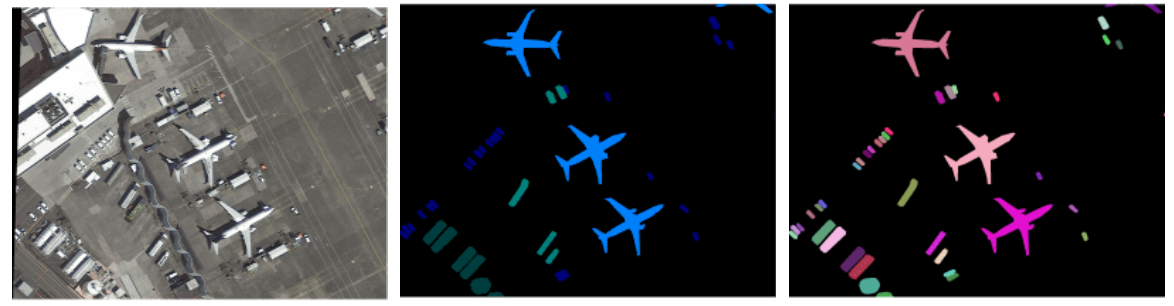
\includegraphics[width=0.8\textwidth]{Images/isaid_examples.png}
\caption{iSAID dataset examples showing instance segmentation and semantic segmentation annotations for aerial imagery.}
\label{fig:isaid_examples}
\end{figure}

[Reference to LoveDA dataset] % \cite{placeholder_loveda}

\begin{figure}[htbp]
\centering
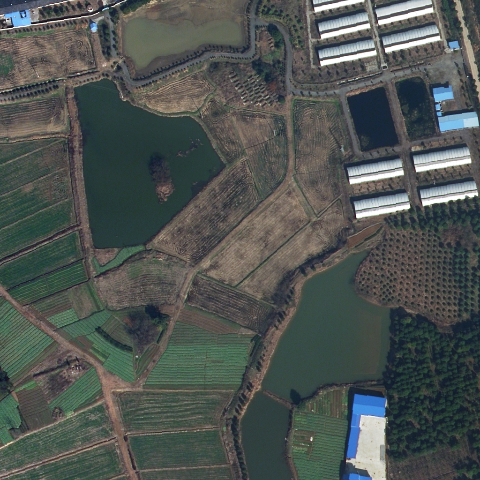
\includegraphics[width=0.8\textwidth]{Images/loveda.png}
\caption{LoveDA dataset examples showing semantic segmentation annotations for land use and land cover classification in aerial imagery.}
\label{fig:loveda_examples}
\end{figure}

[Reference to Potsdam and Vaihingen semantic segmentation datasets] % \cite{placeholder_potsdam} \cite{placeholder_vaihingen}

[Reference to RefSegRS referring segmentation dataset] % \cite{placeholder_refsegrs}

[Reference to RRSIS-D dataset] % \cite{placeholder_rrsis_d}

\begin{figure}[htbp]
\centering
\subfigure[RefSegRS dataset example samples.]{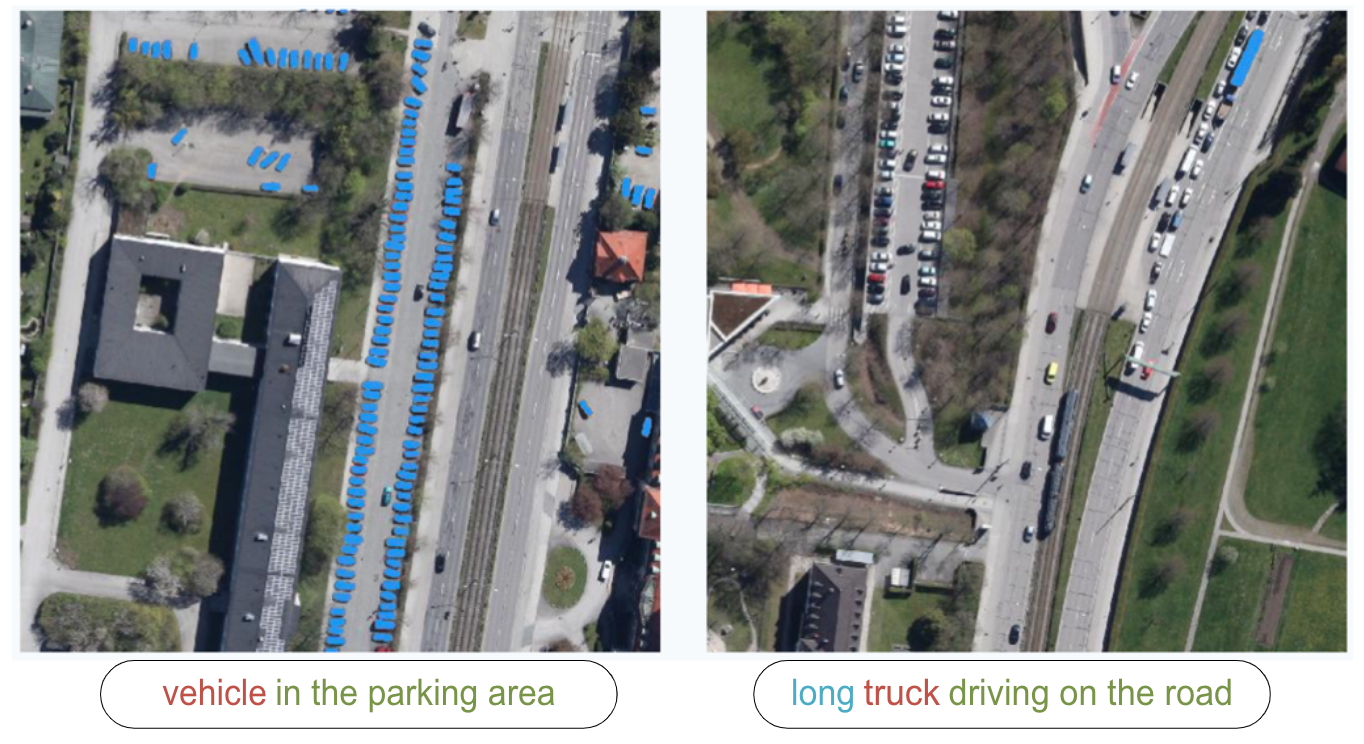
\includegraphics[width=0.45\textwidth]{Images/refsegrs.png}\label{fig:refsegrs}}
\hfill
\subfigure[RRSIS-D dataset example samples.]{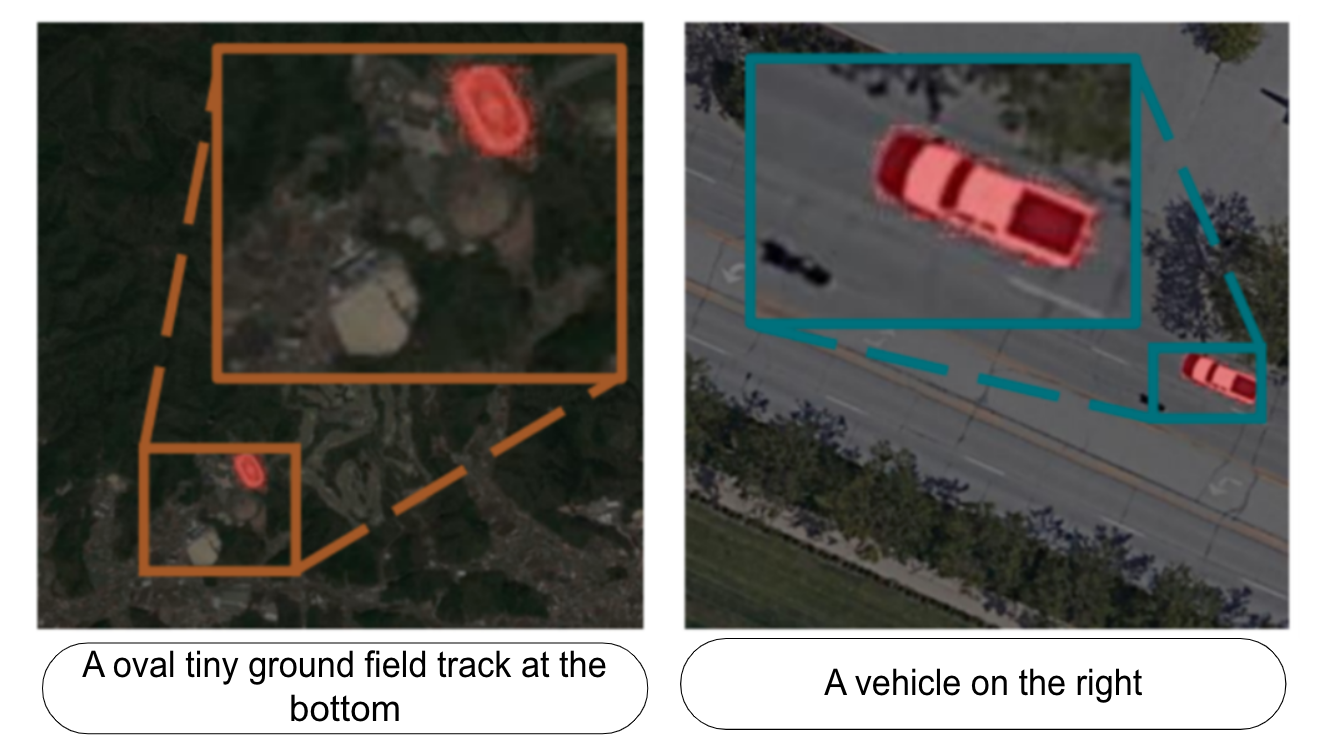
\includegraphics[width=0.45\textwidth]{Images/rrsisd.png}\label{fig:rrsisd}}
\caption{Examples from aerial referring segmentation datasets showing diverse referring expressions with corresponding images and ground truth masks.}
\label{fig:aerial_datasets}
\end{figure}

[Reference to NWPU-Refer dataset] % \cite{placeholder_nwpu}

[diagram for NWPU-Refer dataset example samples]

\begin{table}[htbp]
\centering
\caption{Aerial Referring Segmentation (RRSIS) Dataset Comparison}
\label{tab:rrsis_comparison}
\begin{tabular}{@{}llll@{}}
\toprule
\textbf{Feature} & \textbf{RefSegRS} & \textbf{RRSIS-D} & \textbf{NWPU-Refer} \\
\midrule
Size & 4,420 triplets & 17,402 triplets & 49,745 triplets \\
Source & SkyScapes & RSVGD & Multi-source global \\
Annotation & Manual & Semi-auto (SAM) & Manual \\
Resolution & Limited & 800×800 fixed & 1024-2048px \\
Focus & RRSIS & RRSIS & RRSIS \\
Categories & - & 20 & 32 \\
Attributes & 3 & 7 & 6 dimensions \\
\bottomrule
\end{tabular}
\end{table}

\begin{table}[htbp]
\centering
\caption{Source Aerial Dataset Comparison}
\label{tab:source_comparison}
\begin{tabular}{@{}lll@{}}
\toprule
\textbf{Feature} & \textbf{iSAID} & \textbf{LoveDA} \\
\midrule
Size & 655,451 instances & 5,987 images \\
Source & DOTA (re-ann.) & Spaceborne (0.3m) \\
Annotation & Professional & Manual \\
Resolution & High res. & 1024×1024px \\
Focus & Instance Seg. & Land-cover Seg. + UDA \\
Categories & 15 & 7 \\
Attributes & - & Domain labels \\
\bottomrule
\end{tabular}
\end{table}

\begin{table}[htbp]
\centering
\caption{RRSIS Dataset Split Statistics}
\label{tab:rrsis_splits}
\begin{tabular}{@{}llllll@{}}
\toprule
\textbf{Dataset} & \textbf{Total} & \textbf{Training} & \textbf{Validation} & \textbf{Test} & \textbf{Unit} \\
\midrule
RefSegRS & 4,420 & 2,172 (49.1\%) & 431 (9.8\%) & 1,817 (41.1\%) & expressions \\
RRSIS-D & 17,402 & 8,701 (50.0\%) & 3,480 (20.0\%) & 5,221 (30.0\%) & triplets \\
NWPU-Refer & 49,745 & 34,821 (70.0\%) & 4,974 (10.0\%) & 9,950 (20.0\%) & triplets \\
\bottomrule
\end{tabular}
\end{table}

\begin{table}[htbp]
\centering
\caption{Source Dataset Split Statistics}
\label{tab:source_splits}
\begin{tabular}{@{}llllll@{}}
\toprule
\textbf{Dataset} & \textbf{Total} & \textbf{Training} & \textbf{Validation} & \textbf{Test} & \textbf{Unit} \\
\midrule
iSAID & 2,806 & 1,403 (50.0\%) & 468 (16.7\%) & 935 (33.3\%) & images \\
LoveDA & 5,987 & 2,522 (42.1\%) & 1,669 (27.9\%) & 1,796 (30.0\%) & images \\
\bottomrule
\end{tabular}
\end{table}

% #############################################################################
\section{Segmentation Models for Aerial Images}

This section examines the landscape of segmentation models specifically designed for or applicable to aerial imagery analysis, encompassing both semantic segmentation approaches and referring segmentation techniques.

\subsection{Semantic Segmentation Models}

Foundational vision models provide the backbone architectures for aerial image segmentation tasks through powerful feature extraction and mask generation capabilities.

Vision-language models such as CLIP establish crucial connections between visual and textual modalities through contrastive learning, enabling zero-shot classification capabilities that transfer effectively to aerial imagery domains. The learned joint embedding spaces capture semantic relationships that prove valuable for understanding aerial scene content and object categories.

SigLIP represents an advancement in vision-language training methodologies, improving upon CLIP's contrastive approach through more efficient training objectives and enhanced representation learning. These improvements translate to better performance on downstream aerial image understanding tasks where precise visual-textual alignment is critical.

The Segment Anything Model (SAM) provides a foundational approach to semantic segmentation through its prompt-based architecture, as illustrated in Figure~\ref{fig:sam_architecture}. SAM's design incorporates an image encoder that processes input imagery into rich feature representations, a prompt encoder that handles various input modalities including points, boxes, and text, and a mask decoder that generates precise segmentation boundaries. This architecture demonstrates remarkable generalization capabilities across diverse image domains, including aerial imagery, where its ability to process multiple prompt types enables flexible segmentation workflows that can adapt to different user requirements and annotation strategies.

\begin{figure}[htbp]
\centering
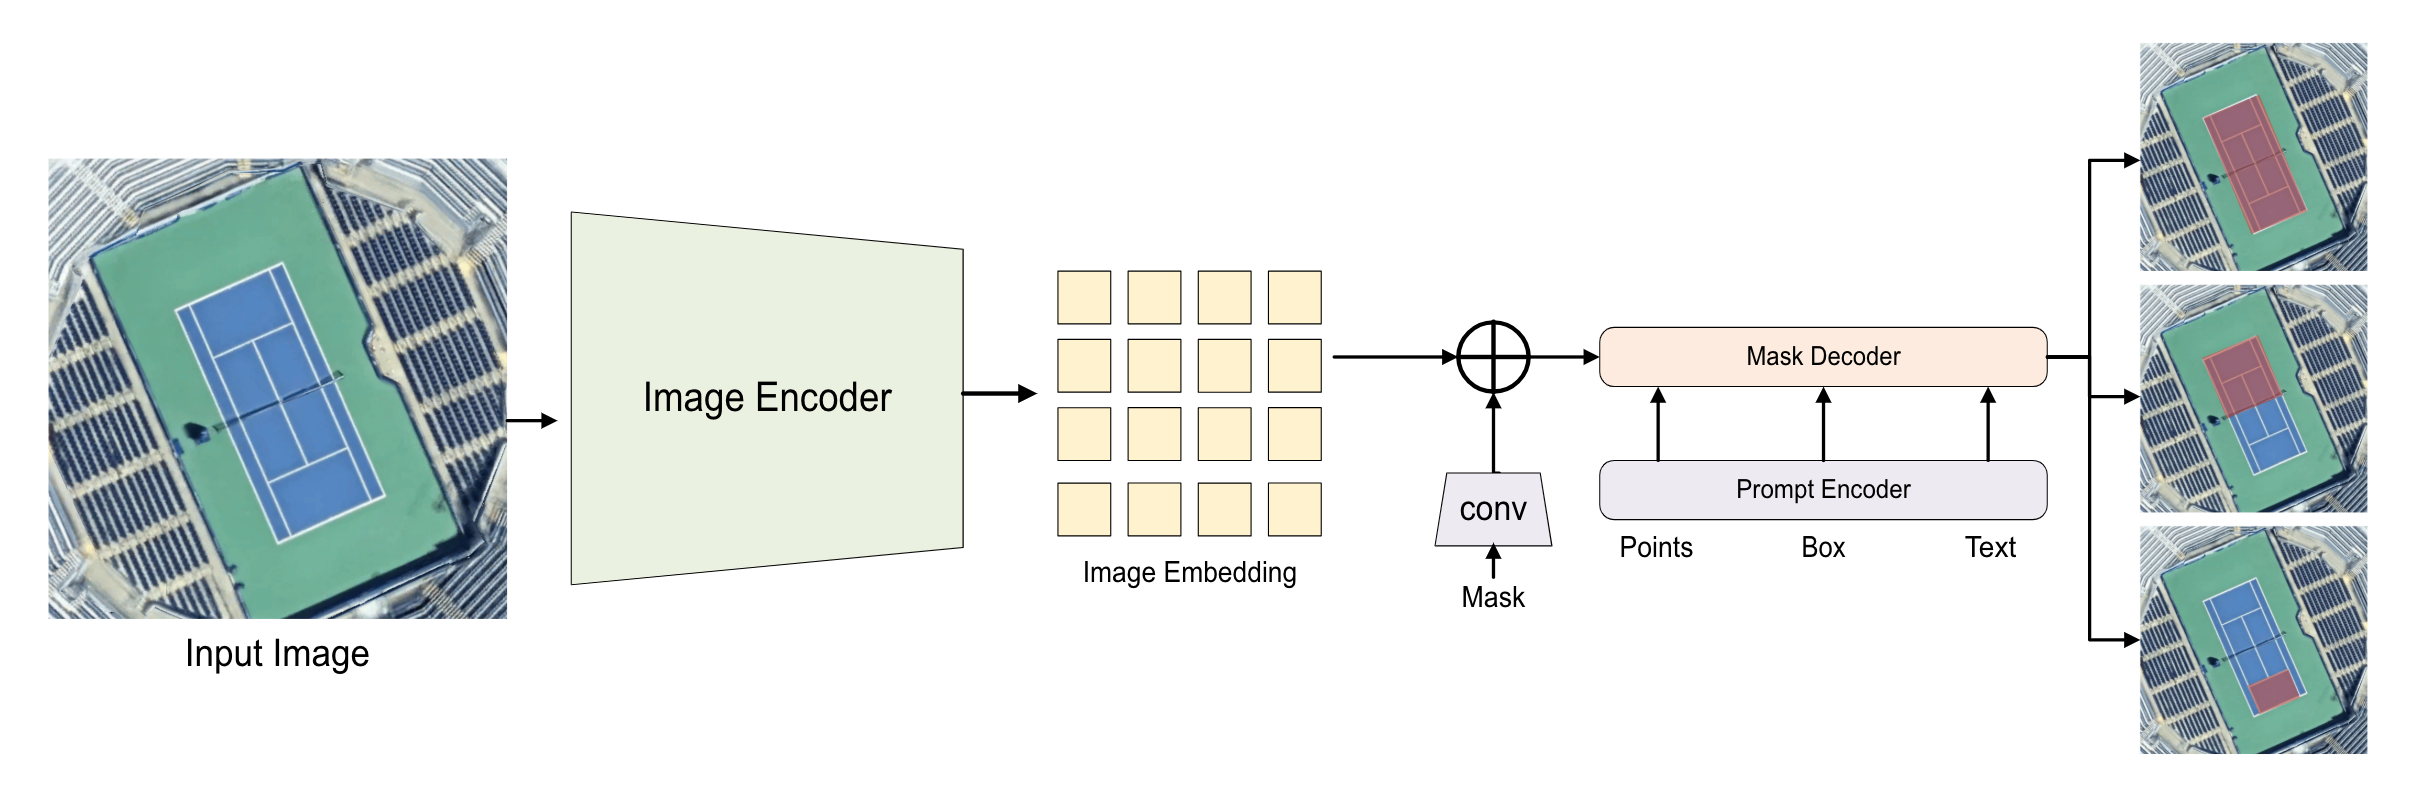
\includegraphics[width=1.0\textwidth]{Images/sam.png}
\caption{Segment Anything Model (SAM) architecture showing the image encoder, prompt encoder, and mask decoder components. The model processes various prompt types including points, boxes, and text to generate precise segmentation masks.}
\label{fig:sam_architecture}
\end{figure}

\subsection{Referring Segmentation Models}

Advanced referring segmentation approaches combine semantic understanding with natural language comprehension to enable text-guided segmentation in aerial imagery contexts.

Previous approaches to language-guided segmentation have established important foundations for referring segmentation in natural images. LAVT introduces attention-based fusion mechanisms that align textual and visual features for precise object localization and segmentation. RMSIN advances multi-scale integration strategies that capture objects at different scales and resolutions. FIANet demonstrates the effectiveness of feature interaction architectures that enable sophisticated text-visual reasoning for segmentation tasks.

RSRefSeg represents a specialized approach designed specifically for aerial referring segmentation, as shown in Figure~\ref{fig:rsrefseg_architecture}. The architecture integrates SigLIP2 vision-language encoders with SAM mask decoders through custom prompter networks that process text-guided segmentation requests. The dual-pathway design processes both local token-level and global sentence-level text-visual interactions, generating sparse and dense prompts that enable precise aerial image segmentation guided by natural language descriptions. This architecture addresses the unique challenges of aerial imagery analysis, including varied object scales, complex spatial relationships, and domain-specific terminology requirements.

\begin{figure}[H]
\centering
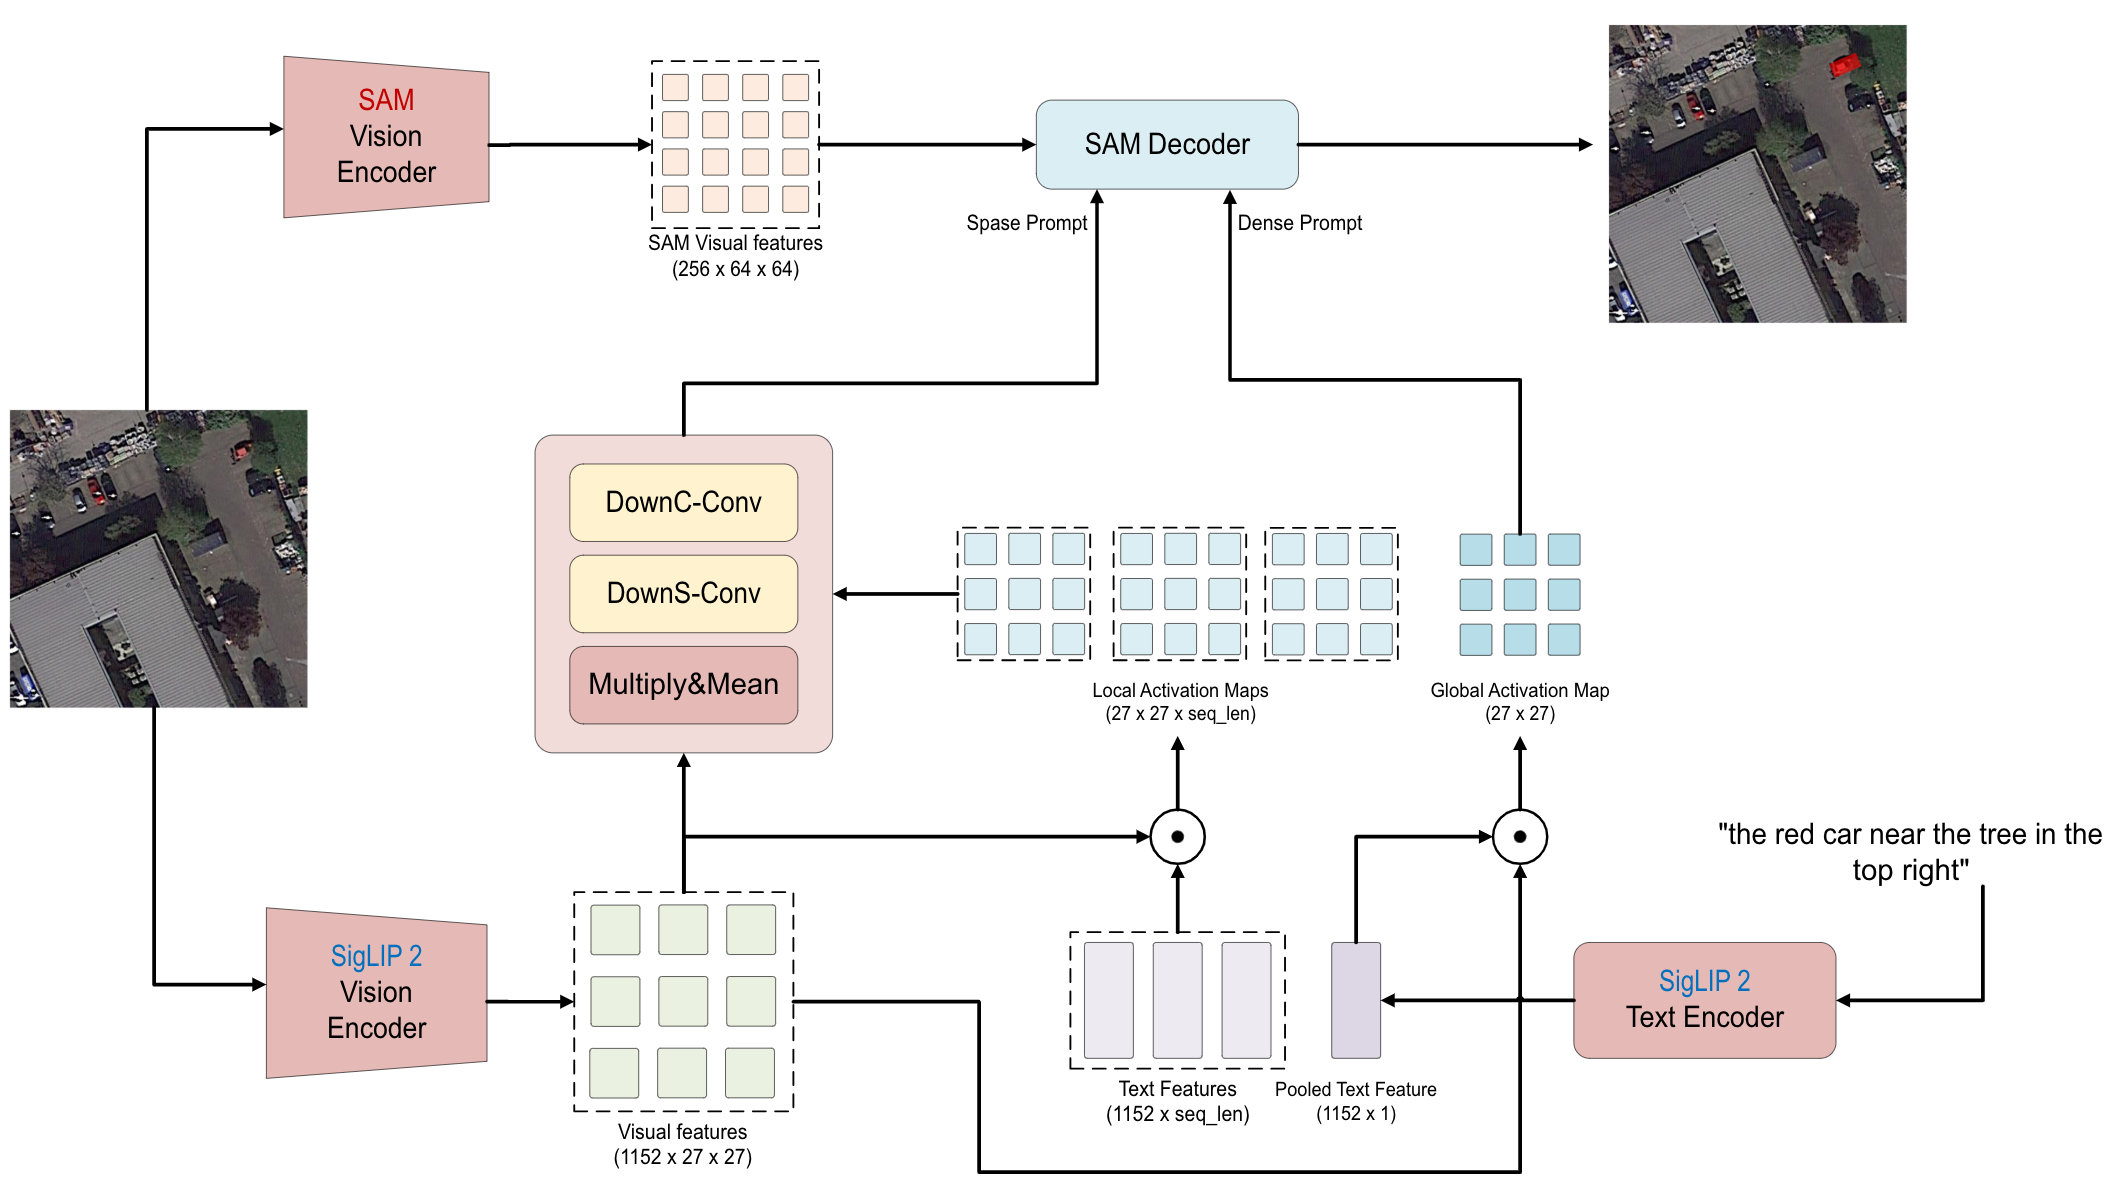
\includegraphics[width=\textwidth]{./Images/clipsam.png}
\caption{RSRefSeg architecture overview showing the integration of SigLIP2 vision-language encoder with SAM mask decoder through custom prompter networks for text-guided segmentation. The dual-pathway design processes both local (token-level) and global (sentence-level) text-visual interactions to generate sparse and dense prompts for precise aerial image segmentation.}
\label{fig:rsrefseg_architecture}
\end{figure}

% #############################################################################
\section{Overview}

[Synthesis of all related work - gaps identified and how this work addresses them] % \cite{placeholder_synthesis}